\documentclass{article}
\usepackage[utf8]{inputenc}
\usepackage{float}
\usepackage{amsmath,amssymb}
\DeclareMathOperator{\E}{\mathbb{E}}
\DeclareMathOperator{\R}{\mathbb{R}}
\newtheorem{theorem}{Theorem}[section]
\usepackage{natbib}
\usepackage{graphicx}

\title{Math 690/Convolution neural network}
\author{Sciber: Guangshen Ma}
\date{11/15/2017}

\begin{document}

\maketitle

\section{Review and guideline}
On previous class, we mention the following concepts:
\begin{itemize}
\item Classifier(supervised):
\item AE:Autoencoder(unsupervised)
\end{itemize}
We talk about the fundamental analysis in machine learning including approximation as well as generalization and we will focus on the Autoencoder method and stability analysis of CNN(convolution neural network). Autoencoder is used for unsupervised learning(without label) and its main goal(in short) is for reconstruction. The stability analysis is to discuss the relationship between the weight parameters and stability of the CNN method. The main topics for this class is in the following:
\begin{itemize}
\item Autoencoder and its architecture
\item Stability analysis of Convolution neural network
\item Approximation theory
\item Generalization analysis of the supervised learning model
\end{itemize}

\section{Autoencoder}
\subsection{Basic architecture}
For the goal of supervised learning(given original data and label), we want to find the function $f(x) = y$ with the probability $p(y) = 1$(We want the model to learn the distribution). For unsupervised learning, we are only given $\overrightarrow{x}$, and we want to learn the distribution of $f(x)$ itself by only given the original data, without label.
\noindent
For the Autoencoder, we are given $\overrightarrow{x}$ and the process is shown in the following:
\begin{itemize}
\item Encode: reduce the dimension(we can think it as the process of extracting feature)
\item Decode: increase the dimension and reconstruct the data
\end{itemize}
We can consider the whole process as encoding and decoding or mapping. The final goal is develop an architecture that can extract important features and use these features to represent the data(reconstruction).

\noindent
The general architecture is shown in the following:
\begin{figure}[H]
\centering
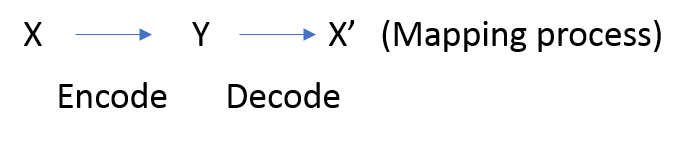
\includegraphics[scale=0.5]{AE_process.png}
\caption{The autoencoder process}
\label{fig:univerise}
\end{figure}

More specifically, this is the architecture of autoencoder method:
\begin{figure}[H]
\centering
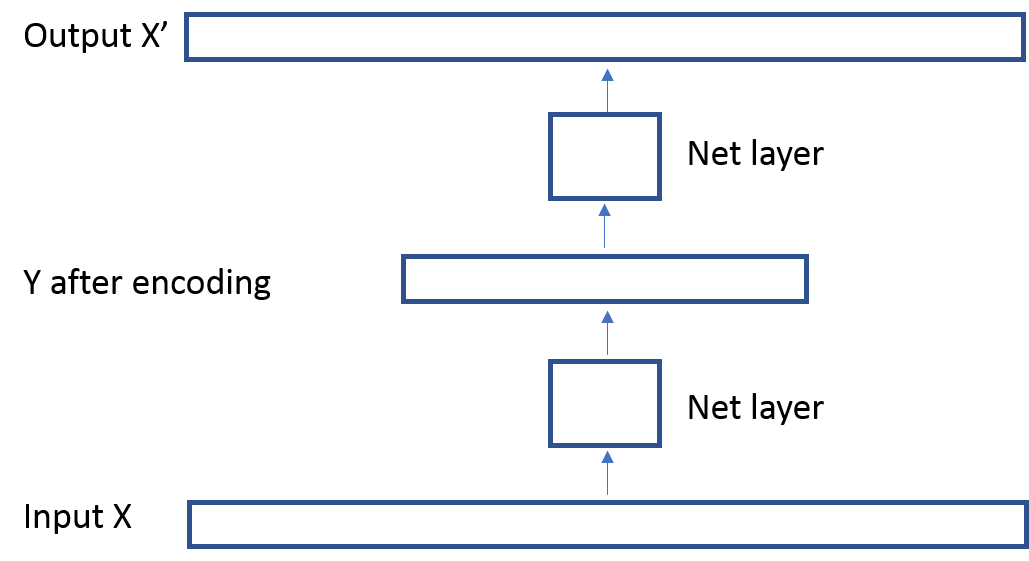
\includegraphics[scale=0.3]{AE_arc.png}
\caption{The autoencoder process}
\label{fig:univerise}
\end{figure}
\noindent
For the above architecture network, we generate the parameter basis for encoding and decoding process with $E_{\theta}$ and $D_{\phi}$ respectively. The representation for mapping based on the network parameter for each layer is:
%\[
%E_{\theta}: \R^{\frac{n(n-1)}{2}
%\]
\[
E_{\theta}:\R^{dx}{\rightarrow}\R^{dy};~D_{\phi}:\R^{dy}{\rightarrow}\R^{dx}
\]
\subsection{Loss function analysis}
The basic question for this model is how to analyze the training loss.Suppose we have training data ${x_i}_{i=1}^{n=t_r}$:
\[
x' =D_{\phi}(E_{\theta}(x)) = D_{\phi}E_{\theta}(x)
\]
Where $x'$ is the output for the network model, as shown before. Then we define the loss function with square $L_2$ norm to measure the difference between training data $x_i$ and output $x_c$ of the model;
\[
Loss = \sum_{i=1}^{n_{tr}}||x_i - D_{\phi}E_{\theta}(x_c)||_2^2
\] 
Remark: The denoising problem of Autoencoder. 

\noindent
Suppose we have the noisy data(Gaussian noise) for the input $\overline{x}$:
\[
\overline{x} = x_i + \sigma_i
\]
The loss function for the noisy data is:
\[
Loss_{noise} = \sum_i||x_i - D_{\phi}E_{\phi}(x_i + \sigma_x)||^2_2
\]
The main question here may be why we need to analyze the noisy problem for Autoencoder. The main goal is to improve the generalization (prevent overfitting) of the whole model by adding noise for input data, so that the model can not only adapt to the training data itself, but also the data around, i.e the model can classify the data points and the surrounding data points(That is the goal of generalization).[ref:Bishop 96']\\

\noindent
The mathematical analysis of the noisy method(as mentioned above):

\noindent
Suppose $f(\overline{x})$ is not changing frequently around $x=\overline{x}$, then we have the Taylor expansion:
\[
f(x_i + \sigma_i) = f(x_i) + f'(x_i)\sigma_i + \frac{1}{2}f''(x_i)\sigma_i^2 + o(|\sigma_i|^n)
\]
Where n denotes the order of higher order term and $\sigma_i$ is gaussian noise.For the term $ f'(x_i)\sigma_i + \frac{1}{2}f''(x_i)\sigma_i^2 + o(|\sigma_i|^n)$, we can consider it as a regularization term for the model(can consider as add a noise term), and so autoencoder by adding noise can be considered as a way to improve the performance of regularization(The reason we add noise for the input sometimes).

\subsection{Approximation theory}
First, let us start with an simple example in supervised learning to discuss the approximation theory. we want to find the function:
\[
y = f(x)
\] 
We want to find $f(\theta)$($\theta$ is the parameter in the model) to approximate f. We want to talk about the case $y{\in}\R$(y being in one dimension). And the target is actually mapping from d dimension to one dimension, as shown in the following:
\[
R^d \rightarrow R,~d=d_x
\] 
We can consider the above case as a simple setting for supervised learning(binary classification problem). We want to talk about the shallow network(one hidden layer) for above case.
\begin{figure}[H]
\centering
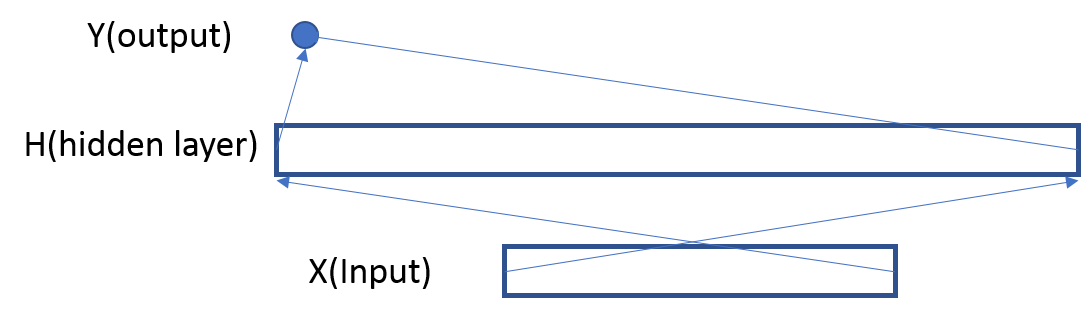
\includegraphics[scale=0.3]{hidden_layer_model.png}
\caption{The supervised learning network with one hidden layer}
\label{fig:univerise}
\end{figure}
For the approximation analysis, we want to find the best parameters $\theta$ that can approximate the function $f$. The goal is:
\[
||f_{\theta} - f|| < C
\]
Where $C$ is the target constant that we want to make it bounded with the conditions from parameters.\\
\noindent
Suppose $f_m$ is the approximated function with m neurons, then we have:
\[
||f_m - f|| < \epsilon
\]
Where m is large enough and $\epsilon$ is a small constant.\\
\noindent
Based on the history of machine learning, we have two traditional results (Only refer the results without details and proving here):
\begin{itemize}
\item $\epsilon$ can be arbitrarily small and m is exponentially large to approximate any continues f [ref:Hormit'89,Gylenko'89]
\item $||f_m - f||^2_2 {\leq} \frac{c_f}{m}$ where $c_f$ is the Fourier criterion and m is the number of neurons [ref:Barron 93',94].
\end{itemize}
Then the question lies in how we determine the coefficients $c_f$ and m. \\
\noindent 
More specifically, we have the representation for f:
\[
c_f = \int_{R^d}||w|||f'(w)|dw < +{\infty}
\]
Where the barron function $f$ is 
\[
f:~B \rightarrow \R~ B:~unit~ball(for~this~case)~in~\R ^d,~B = \{ x,~||x||{\leq}1 \}
\]
Where f has the Fourier transform $\widehat{f}(w)$ and we have the inverse transform:
\[
f(x) = f(0) + \int_{R^d}(e^{iw^Tx} - 1) \widehat{f}(w)dw 
\] 
Also, $c_f<+\infty$.
Based on the above theory, we will continue by discussion of approximation theory in supervised learning.\\
\noindent
Recall the network structure~$(x{\in}R^d,h{\in}R^m,y{\in}R^1)$. The first output after the hidden layer:
\[
h_R(x) = \sigma(\alpha_k^Tx + b_k)
\]
Where $\alpha_k {\in} \R^d$, $b_k {\in} \R$,~$k=1,2,{\cdots}m$.
We also have the output $y$: 
\[
y(h) = \sum_{k=1}^m c_kh_k + c_0
\]
Then we have (m is the number of neurons):
\[
f_m(x) = c_0 + \sum_{k=1}^m c_k\sigma(\alpha_k^Tx+b_k)
\]
Where the $\sigma$ is the sigmoid function, $c_k$ is the weight on the second layer. We then come up with a theorem:
\begin{theorem}
Suppose $f$ is Barron function with $c_f<+\infty$, then $\forall \mu$, we have $\forall \sigma$ sigmoid function, $\forall m {\geq} 1$, $\exists \{ \alpha_k,b_k,c_k \}_k$ s.t f can be approximated by $f_n$ of the form that satisfies $\int_B |f(x) - f_m(x)|^2d \mu (x){\leq} \frac{(2c_f)^2}{m}$ 
\end{theorem}
However, the question lies in how big is the coefficient $c_k$. Particularly, we have [reference from paper without details here]:
\[
c_0 = f(0),~\sum_{k=1}^m |c_k| {\leq} 2c_f
\] 

\subsection{Generalization analysis} 
We want f to be generalizable given that the model can be applied to other data rather than only the training data. We first introduce the generalization error:
\[
L_R(f_{\theta}) = \E \limits_{x \sim p_x} |f_{\theta} - f(x)|^2
\]
Where $L_R$ is the expected loss or population error. 
\noindent
We also have the training loss:
\[
\widehat{L}_{R}[f_{\theta}] = \frac{1}{n_{tr}}\sum_{i=1}^{n_{tr}}|f_{\theta}(x) - f(x)|^2
\]
We want to find the gap between expectation loss and training loss.
\[
gap = L_R(f_{\theta}) - \widehat{L}_{R}[f_{\theta}]
\]
One question for this problem is that can we use simple concentration argument for this problem, as we discussed before, so that we can easily control the gap. That is to say can we use concentration method to bound or control the loss.\\

\noindent
However, they(The two loss) cannot be considered as independent since they are not independent for the training data so that not concentration methods can be used here(they cannot be considered independent), as shown in the following. Suppose $\widehat{\theta}$ is trained from $x_{tr} = \{ x_i \} ^{n_{tr}}_{i=1}$, and we have:
\[
\widehat{R_n}[f(\widehat{\theta})] = \frac{1}{n} \sum_{i=1}^n |f_{\widehat{\theta}}(x_i) - f(x_i)|^2
\]
The $\widehat{\theta}$ from the $f_{\widehat{\theta}}(x_i)$ is actually depending on $x_{tr}$. That is the reason we cannot use concentration strategy here.

\section{Note}
\begin{itemize}
\item ReLu and sigmoid functions are not fully discussed for this note. 
\item Some details or build-in theory are referred from the papers and the details (such as prove or demonstration) are not provided here.
\end{itemize}



\end{document}


There is a theory which states that if ever anyone discovers exactly what the Universe is for and why it is here, it will instantly disappear and be replaced by something even more bizarre and inexplicable. There is another theory which states that this has already happened.

%\begin{figure}[h!]
%\centering
%\includegraphics[scale=1.7]{universe.jpg}
%\caption{The Universe}
%\label{fig:univerise}
%\end{figure}

\section{Conclusion}
``I always thought something was fundamentally wrong with the universe'' \citep{adams1995hitchhiker}





\bibliographystyle{plain}
\bibliography{references}